\documentclass{article}
\usepackage{graphicx}
\usepackage{amsmath}
\usepackage{hyperref}
\usepackage{cite}
\usepackage{listings}
\usepackage{xcolor}

\lstset{
    language=Python,             % Specify Python as the language
    basicstyle=\ttfamily,        % Use monospaced font for code
    keywordstyle=\color{blue},   % Color for keywords
    commentstyle=\color{gray},   % Color for comments
    stringstyle=\color{red},     % Color for strings
    numbers=left,                % Line numbers on the left
    numberstyle=\tiny\color{gray}, % Style for line numbers
    stepnumber=1,                % Number every line
    frame=single,                % Frame around the code
    breaklines=true              % Enable line breaking
}

\graphicspath{{project/paper_images/}}

\title{Deep Learning Project}
\author{
    Group Members: \\
    Farooq Mahmud
}
\date{September 20, 2024}

\begin{document}

\maketitle

\section{Introduction}
Deep learning models, particularly Convolutional Neural Networks, have made great strides in solving complex computer vision tasks such as image classification. Among the key advancements in this area is the Inception architecture, introduced by Szegedy et al. (2015) in the paper "Going Deeper with Convolutions." This architecture was designed to balance computational efficiency with improved classification accuracy. This architecture achieved winning results in the ImageNet Large-Scale Visual Recognition Challenge (ILSVRC) in 2014. The primary innovation of the Inception architecture is its use of multi-scale feature extraction and dimensionality reduction, which allows it to increase network depth and width without excessive computational overhead\cite{szegedy2015going}.

This paper aims to replicate the results presented by Szegedy et al., critically assess the impact of the Inception architecture, and test its performance on an alternative dataset. We attempt to reproduce the GoogLeNet model by writing our own Python implementation using the Tensorflow library. Our implementation is evaluated on both a subset of the ImageNet dataset and a secondary dataset, CIFAR-10, to assess its generalization capability. Through this replication and exploration, we seek to validate the core contributions of the Inception model, gain a deeper undertanding of convolutional neural networks, and an appreciation of the associated challenges.


\section{Background}

GoogLeNet introduced a novel approach to convolutional neural networks by stacking multiple Inception modules. Each Inception module consists of parallel branches that apply different-sized convolutional filters (1x1, 3x3, 5x5) and max-pooling operations in parallel. These branches are concatenated to capture multi-scale features.

The Inception module aims to mitigate computational costs by including 1x1 convolutions for dimensionality reduction before performing the larger convolution operations. This was one of the key innovations that made GoogLeNet both efficient and powerful, despite being deeper than previous CNN architectures such as AlexNet and VGGNet~\cite{krizhevsky2012imagenet, simonyan2015vgg}.

\subsubsection{Inception Architecture}
The Inception architecture was introduced to address two primary challenges in CNNs: improving model accuracy while maintaining computational efficiency. Szegedy et al. proposed a novel structure called the Inception module, which incorporates parallel convolutional filters of different sizes (1x1, 3x3, and 5x5) along with max-pooling. The key advantage of this approach is that it allows the network to capture features at multiple scales simultaneously, enhancing the model's ability to learn complex spatial hierarchies within images.

Another major innovation was the use of 1x1 convolutions for dimensionality reduction. By applying 1x1 filters before 3x3 and 5x5 convolutions, the Inception module significantly reduces the number of parameters and computational cost without sacrificing accuracy. This strategy enables the network to be deeper and wider without a substantial increase in computational complexity.

The Inception architecture was implemented in a 22-layer deep network, GoogLeNet, which was used to win the ILSVRC 2014 competition. As Figure \ref{fig:googlenet-comp-perf} shows, GoogLeNet has the lowest top-5 error rate compared to previous winners~\cite{szegedy2015going}.

\begin{figure}[ht]
    \centering
    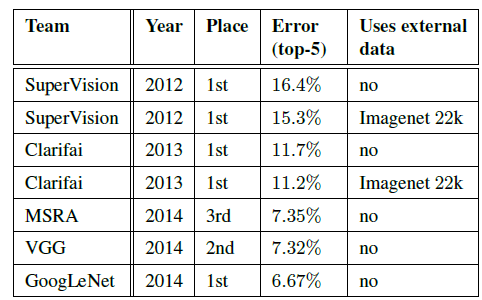
\includegraphics[scale=0.7]{project/paper_images/googlenet_competition_perf.png}
    \caption{GoogLeNet performance at ILSVRC 2014}
    \label{fig:googlenet-comp-perf}
\end{figure}


\section{Methodology}

\subsection{Image Selection}
The Imagenet dataset contains over 1 million images with a size of over 1TB. Processing this amount of data would not be practical given the available coumputing power. In order to make processing possible in a reasonable timeframe, a subset of the Imagenet images was downloaded. The subsets, or \textit{synsets} map to the CIFAR-10 image classes as shown in Table \ref{tab:synsets}.

\begin{table}[ht]
    \centering
    \begin{tabular}{ll}
    \hline
    \textbf{Synset ID} & \textbf{Equivalent CIFAR-10 Class} \\ \hline
    n02691156 & airplane \\ \hline
    n02958343 & automobile \\ \hline
    n01503061 & bird \\ \hline
    n02121808 & cat \\ \hline
    n02419796 & deer \\ \hline
    n02084071 & dog \\ \hline
    n01641577 & frog \\ \hline
    n02374451 & horse \\ \hline
    n04194289 & ship \\ \hline
    n04467665 & truck \\ \hline
    \end{tabular}
    \caption{Imagenet synset to CIFAR-10 class mapping}
    \label{tab:synsets}
\end{table}

The resulting download consists of 14,738 files with a total size of 1.3GB. Scaling the images to 224 x 224 pixels, the dimensions used by Szegedy, et. al. decreased the size to a manageable 137MB.

After scaling, 100 images from each class were set aside to use for evaluating the trained model.

Training and validation sets were created in-situ using Tensorflow's \textt{image\_dataset\_from\_directory} function. The percentages were 80\% for training, and 20\% for validation.

The networks mentioned in this report were training on an NVIDIA Quadro P2000 GPU having 5GB of dedicated memory.

\subsection{A Simplified GoogLeNet Network}
Before constructing a complex model like GoogLeNet, it is a good idea to use a simple network as a baseline. This network is shown in Figure \ref{fig:cnn-simple}. This network is conceptually similar to GoogLeNet but without the complexity of the Inception modules. At it's core, the GoogLeNet architecture stacks multiple convolutional layers before downsampling through pooling. Stacking multiple layers helps networks capture progressively more complex features, improves generalization, and increases performance while keeping computational cost from getting out of hand. This is a common design pattern in many successful image classification networks\cite{simonyan2014very}.

The architecture of this network was informed by the following constraints:
\begin{itemize}
    \item 10 image classes versus 1000 image classes in the complete ImageNet dataset.
    \item About 14.7K images instead of the over 1 million images in the complete ImageNet dataset.
\end{itemize}

These constraints were the reason why the filter depths range from 32 to 256.


\begin{figure}[ht]
    \centering
    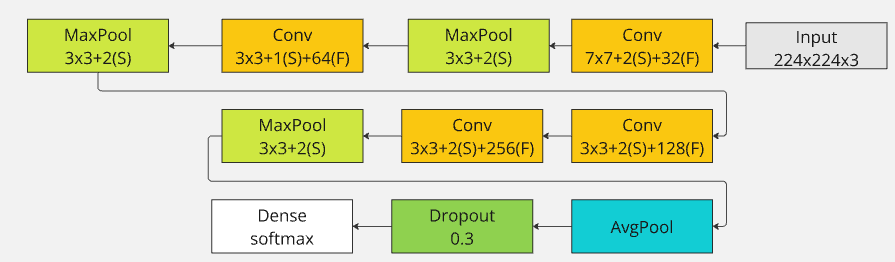
\includegraphics[scale=0.7]{project/paper_images/googlenet_simple.png}
    \caption{Simplified version of the GoogLeNet network}
    \label{fig:cnn-simple}
\end{figure}

This simple model, when trained for 30 epochs, achieved a maximum accuracy of 55.8\% at Epoch 29 as shown in Figure \ref{fig:googlenet-simple-accuracy}.

The validation accuracy and training accuracy track well, indicating a lack of overfitting. Applying data augmentation to the training set mitigates overfitting, especially with the smaller dataset. The augmentation code is shown in Listing \ref{lst:augmentation}

\begin{lstlisting}[caption={Augmentation code}, label={lst:augmentation}]
augmentation = tf.keras.Sequential([
    layers.RandomFlip("horizontal"),
    layers.RandomRotation(0.1),
    layers.RandomZoom(0.2),
])

# Apply the augmentation only on the training dataset
train_dataset = train_dataset.map(lambda x, y: (augmentation(x, training=True), y))
\end{lstlisting}

\begin{figure}[ht]
    \centering
    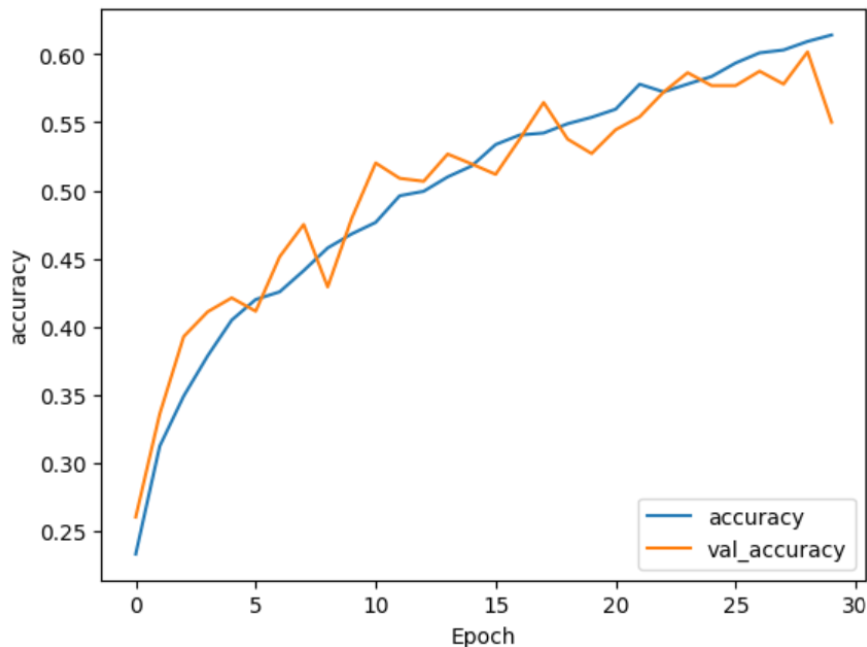
\includegraphics[scale=0.7]{project/paper_images/googlenet_simple_accuracy.png}
    \caption{Accuracy of the simplified version of the GoogLeNet network}
    \label{fig:googlenet-simple-accuracy}
\end{figure}

\subsection{Replicating the GoogLeNet Network}
The GoogLeNet architecture is explained in tabular form in Table 1 in the Szegedy paper and is reproduced in Figure \ref{fig:googlenet-arch}. The introduction of Inception layers having parallel convolutional filters is the primary difference from typical sequential networks. The replication attempt, when trained for 30 epochs, achieved a maximum accuracy of 56.9\%. This is essentialy the same as the simple network. The upshot is that it only took 8 epochs to arrive at the maximum accuracy as shown in Figure \ref{fig:googlenet-complex-accuracy}. Nevertheless, both models are nowhere near the accuracy of the model in the Szegedy paper. Their model achieved a top-5 error rate of only 6.7\%. While the paper does not mention the accuracy, it is not a leap to assume that the accuracy was well above the accuracy in the replication attempt. The network is graphically depicted in Figure \ref{fig:googlenet-complex}

\begin{figure}[ht]
    \centering
    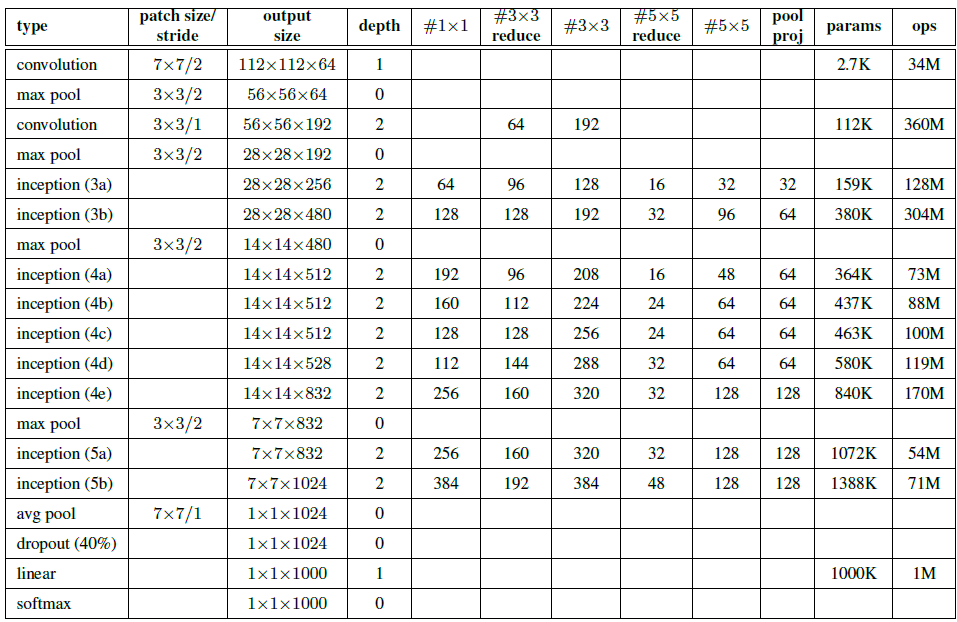
\includegraphics[scale=0.7]{project/paper_images/googlenet_arch.png}
    \caption{GoogLeNet architecture with Inception layers}
    \label{fig:googlenet-arch}
\end{figure}

\begin{figure}[ht]
    \centering
    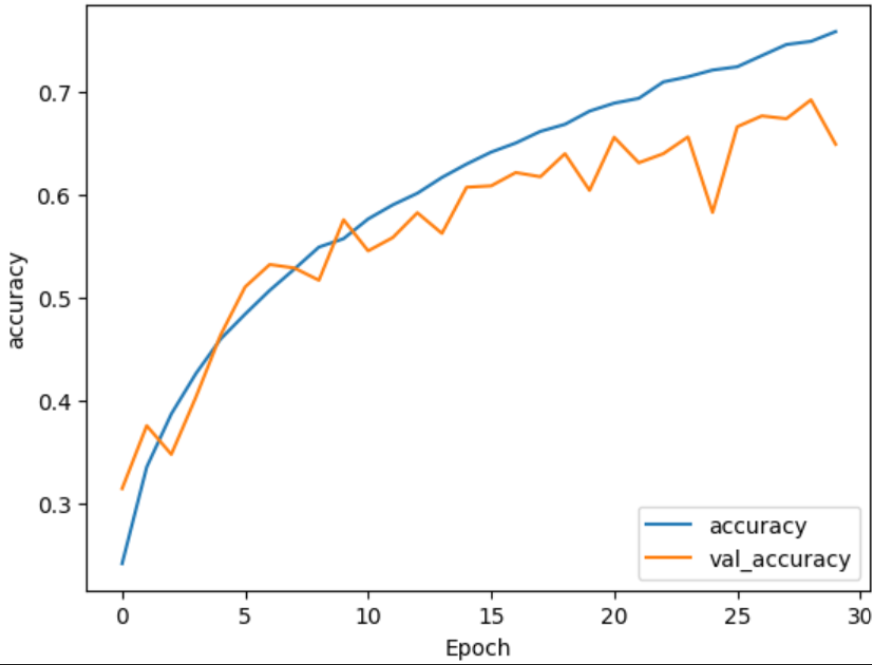
\includegraphics[scale=0.7]{project/paper_images/googlenet_complex_accuracy.png}
    \caption{Accuracy of the simplified version of the GoogLeNet network}
    \label{fig:googlenet-complex-accuracy}
\end{figure}

\begin{figure}[ht]
    \centering
    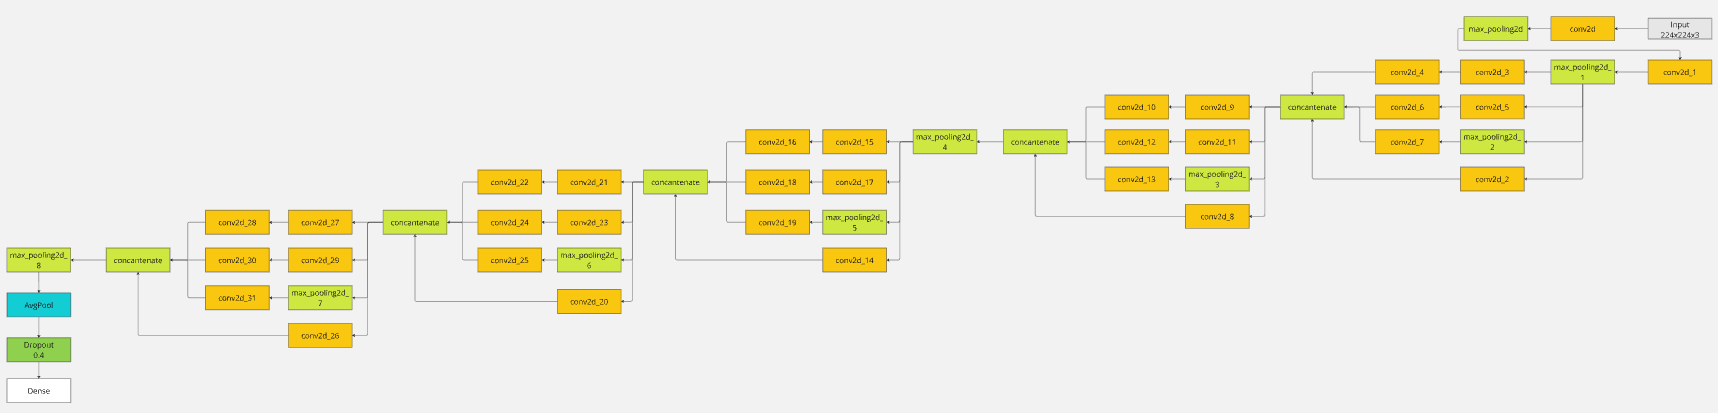
\includegraphics[width=\textwidth]{project/paper_images/googlenet_complex.png}
    \caption{Replicated GoogLeNet network}
    \label{fig:googlenet-complex}
\end{figure}

\subsection{Model Evaluation}
Both networks were evaluated using two sets of images. The first is the 1,000 ImageNet images set aside prior to model training. The second set is sourced from the CIFAR-10 dataset. The CIFAR-10 dataset contains 1,000 32x32 RGB images.

\subsubsection{Performance On Unseen Imagenet Images}

\subsubsection{Performance On CIFAR-10 Images}

\subsection{Challenges}
The Inception architecture's key contribution is its ability to balance computational efficiency with accuracy. By incorporating 1x1 convolutions for dimensionality reduction and parallel convolutions in the Inception modules, GoogLeNet achieves leading performance without increased compute cost or model parameters.

In our reproduction, the model's performance on the ImageNet dataset was not  close to the results reported in the original paper. This is not an indictment on the effectiveness of the architecture, however. Rather, the small dataset size could be a factor. Additionally, our interpretation of the Inception modules to code could have variations from the code used by Szegedy et al.

One of the challenges we encountered was the high computational demand of training, event on the subset of ImageNet images we used. Although GoogLeNet is more efficient than many of its contemporaries, training still required GPU resources. We used data augmentation techniques, such as random cropping, random horizontal flipping, and random zoom to avoid overfitting. We also needed to reduce the learning rate to 0.0001 and reduce batch size to 16 so as not to overwhelm the GPU. The training performance is summarized in Table \ref{tab:training_times}

\begin{table}[ht]
    \centering
    \begin{tabular}{llll}
    \hline
    \textbf{Model} & \textbf{Batch size} & \textbf{Epochs} & \textbf{Training time (minutes)} \\  \hline
    Simple & 16 & 30 & ?? \\ \hline
    Complex & 16 & 30 & 69 \\ \hline
    \end{tabular}
    \caption{Training times}
    \label{tab:training_times}
\end{table}

\subsection{Critical Assessment}
The Inception architecture has had a significant impact on the field of deep learning, particularly in image classification. Its introduction marked a shift from simply increasing the size of models to incorporating more sophisticated designs that optimize the use of computational resources. This focus on efficiency has made the architecture suitable for deployment in resource-constrained environments, such as mobile devices.

The architecture has also influenced subsequent innovations, including more advanced object detection systems like Faster R-CNN and SSD, which build on the principles introduced by Inception. Additionally, later versions of the Inception architecture continue to push the boundaries of accuracy and efficiency in deep learning.

However, the architecture is not without its limitations. Despite its efficient design, training the network still requires significant compute power, especially for large datasets like ImageNet. Furthermore, the design of the Inception module, while effective, introduces additional complexity to the network architecture, making it  challenging to implement and optimize.

\bibliographystyle{plain}
\bibliography{project/refs}

\end{document}
